\documentclass{article}
\usepackage{caption}
\usepackage{subcaption}
\usepackage{graphicx}
\usepackage{tikz}
\usepackage{tikzsymbols}
\usetikzlibrary{calc}
\usepackage{float}
\usepackage{pdflscape}
\usepackage{geometry}
\geometry{a4paper, landscape, margin=1cm}
\pagestyle{empty}

\def\centerarc[#1](#2)(#3:#4:#5){\draw[#1] ($(#2)+({#5*cos(#3)},{#5*sin(#3)})$) arc (#3:#4:#5);}

\begin{document}
	\centering
	\begin{figure}[H]
			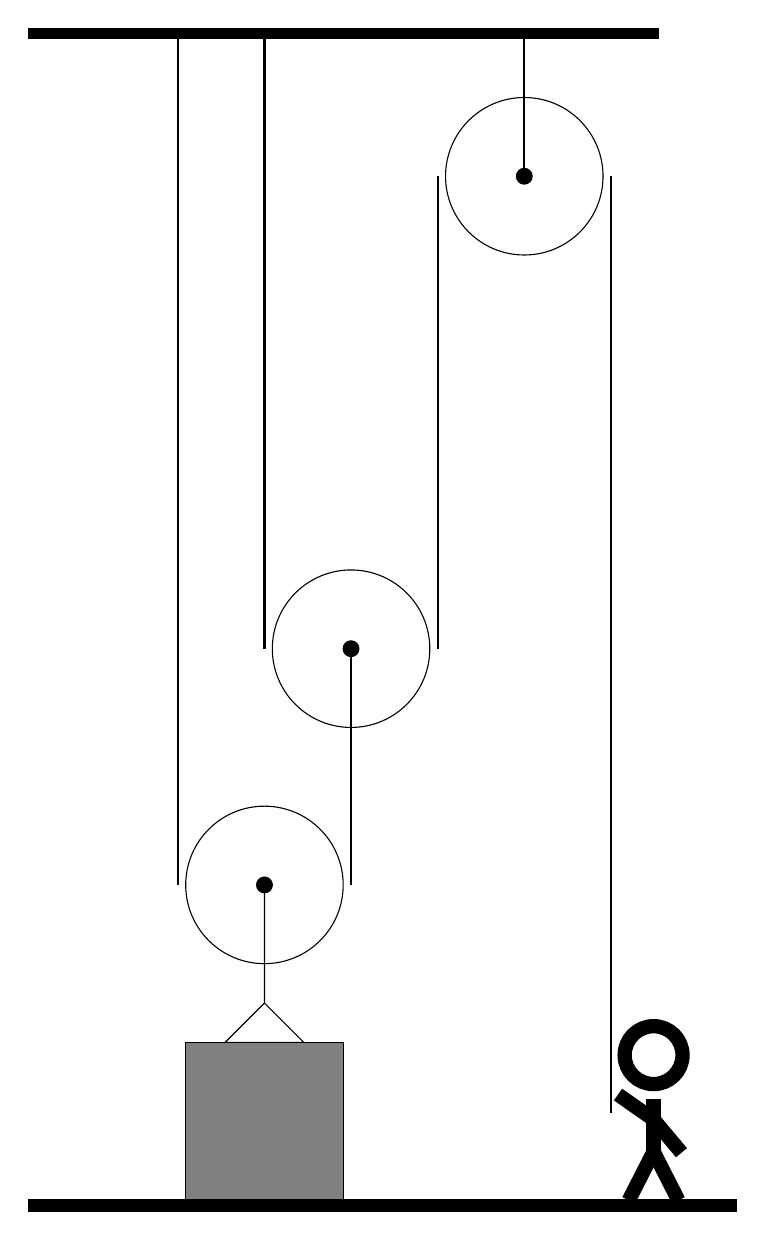
\begin{tikzpicture}
				%%%%% START %%%%%
								
				\draw[fill=black] (-2, 11.75) rectangle (6, 11.88);
				
				\draw (1, 1) circle (1);
				\draw[fill=black] (1, 1) circle (0.1);
				
				\draw (2.1, 4) circle (1);
				\draw[fill=black] (2.1, 4) circle (0.1);
				
				\draw (4.3, 10) circle (1);
				\draw[fill=black] (4.3, 10) circle (0.1);
				\draw[thick] (4.3, 10) -- (4.3, 11.75);
				
				\draw (1, 1) -- (1, -0.5) -- (0.5, -1) -- (1.5, -1) -- (1, -0.5);
				\draw[fill=black!50] (0, -1) rectangle (2, -3);
				
				\draw[thick] (-0.1, 11.75) -- (-0.1, 1);
				\centerarc[thick](1, 1)(180:360:1.1);
				\draw[thick](2.1, 1) -- (2.1, 4);
				\draw[thick] (1.0, 11.75) -- (1.0, 4);
				\centerarc[thick](2.1, 4)(180:360:1.1);
				\draw[thick](3.2, 4) -- (3.2, 10);
				\centerarc[thick](4.3, 10)(0:180:1.1);
				\draw[thick] (5.4, 10) -- (5.4, -1.9);
				
				\node at (5.9, -1.9) {\Strichmaxerl[10][-35][-50]};
				
				\draw[fill=black] (-2, -3) rectangle (7, -3.15);
				%%%%% END %%%%%
			\end{tikzpicture}
	\end{figure}	
\end{document}